\section{Complex geometries}
\label{sec:dsmc_complex_geometries}
All the surface interaction models from section \ref{sec:surface_interactions} use the surface normal and tangent vectors to calculate the reflected velocities. These vectors are easy to determine if the system consists of two parallel plates in the xy-plane, or any other mathematically well described geometry. Such systems are interesting as validation test cases, but most real world materials have a more complex geometry without any simple mathematical description. A very much used representation of such geometries is a triangle mesh in which the surface consists of many connected triangles. The triangles have a well defined normal vector and tangent plane which is easy to calculate. With this method, collision detection is done by checking intersection with each triangle and is rather computationally expensive. In this thesis, we have chosen another approach by representing the system as a large, binary three-dimensional matrix consisting of voxels, each having the value \textit{filled} or \textit{empty}. With this model, collision detection is done by a quick memory lookup to check if the voxel corresponding to the position of a particle is filled or not. In this section we discuss how to create such a matrix, how to identify the surface voxels and how we calculate the normal and tangent vectors. 

\subsection{Binary representation}
\label{sec:dsmc_binary_representation}
Any system geometry is fully described by a three dimensional matrix with dimensions $m\times n\times l$. Each matrix element represents a voxel in the physical space, and can take values 0 or 1. A value of one means that the voxel is filled, whereas zero means the voxel is empty. Since the particles only will collide directly with the voxels defining the surface, these are given the value 2. The idea is best explained with an example.
\subsection{Example - a cylinder}
We will now show how to create a cylinder with radius $r$ with this model. The idea is very simple, we just loop through every voxel in the system and check whether or not the voxel should be marked as filled or empty. We define that no matter how many voxels we have, the radius $r$ is given in the range $[0, 0.5]$ so that the system is a $1\times 1\times 1$ cube. The algorithm should be easy to understand from the code example in listing \ref{lst:dsmc_geometry_cylinder}.
\begin{lstlisting}[caption=An example showing how to create a cylinder., label=lst:dsmc_geometry_cylinder]
void create_cylinder(double radius) {
	float voxel_size_x = 1.0 / num_voxels_x;
	float voxel_size_y = 1.0 / num_voxels_y;

	double cylinder_center_x = voxel_size_x * (num_voxels_x / 2.0);
	double cylinder_center_y = voxel_size_y * (num_voxels_y / 2.0);

	for(int i=0; i<num_voxels_x; i++) {
	    for(int j=0; j<num_voxels_y; j++) {
	        for(int k=0; k<num_voxels_z; k++) {
	            double x = i/double(num_voxels_x) + voxel_size_x/2.0;
	            double y = j/double(num_voxels_y) + voxel_size_y/2.0;
	            bool is_solid = true;

	            double dx = (x - cylinder_center_x);
	            double dy = (y - cylinder_center_y);
	            double dr2 = dx*dx + dy*dy;

	            if(dr2 < radius*radius) {
	                is_wall = false;
	            }

	            int index = i*ny*nz + j*nz + k;

	            if(is_wall) vertices[index] = 1;
	            else vertices[index] = 0;
	        }
	    }
	}

	calculate_normals_tangents_and_inner_points();
}
\end{lstlisting}
Notice the last line there, the function \textit{calculate\_normals\_tangents\_and\_inner\_points()}. After all voxels are marked as filled or empty, we need to identify the surface voxels and calculate their tangent and normal vectors.
\subsection{Identifying the surface voxels}
A voxel that is filled, but not part of the surface, will be completely surrounded by filled voxels. We \textit{define} the surface voxels as \textit{the filled voxels that have less than 26 neighbouring filled voxels}. The algorithm can be implemented like in listing \ref{lst:dsmc_geometry_identify_surface} (we also need to take care of the periodic boundary conditions, but the idea is best illustrated without that complication).
\begin{lstlisting}[caption=An example showing how to identify the surface voxels. The world\_matrix contains all the voxel values (zeros and ones)., label=lst:dsmc_geometry_identify_surface]
bool is_surface(int voxel_index_i, int voxel_index_j, int voxel_index_k) {
	for(int i=-1;i<=1;i++) {
    	for(int j=-1;j<=1;j++) {
			for(int k=-1;k<=1;k++) {
				// Skip self
				if(i == j == k == 0) continue; 

                if(world_matrix[voxel_index_i + i][voxel_index_j + j][voxel_index_k + k] == 0) {
                	// This neighbour is empty, hence a surface voxel
                	return true;
                }
            }
        }
    }

    return false;
}
\end{lstlisting}
This has to be done for every voxel in the system, but only once per geometry. When we have identified all surface voxels, we need to calculate the normal and tangent vectors for each of them. Once this is done, we can save and use the geometry in a simulation.
\subsection{Calculating normal and tangent vectors}
Each surface voxel is a cube with six faces, each having a normal vector pointing out from the cube. Each face then defines the tangent plane orthogonal to this normal vector. When a particle collides with a surface voxel, we can calculate which face the particle passed through and use those vectors to calculate the reflected velocity. However, in this thesis, we have developed a new way of describing the surface vectors. We will use the neighboring voxels so that the normal vector of a surface voxel contains information of the curvature of the surface in order to have more realistic collisions.\\
The idea is simpler to illustrate for a two dimensional square, but the concept can easily be generalized to three dimensions. A square consisting of 9 pixels has a geometric center $\vec r_\text{gc}$, plus a center of mass $\vec r_\text{cm}$ which can be defined by the values, the mass, of the voxels
\begin{align}
	\vec r_\text{cm} = \sum_{i,j} \vec r_{ij}m_{ij},
\end{align}
where $m_{ij} \in \{1,0\}$ and $\vec r_{ij}$ is the coordinate of the voxel with $\vec r_\text{gc}$ as the origin. We \textit{define} the normal vector to be the normalized local center of mass vector
\begin{align}
	\label{eq:dsmc_normal_vector}
	\vec n = \frac{\vec{r_\text{cm}}}{|\vec{r_\text{cm}}|}.
\end{align}
In figure \ref{fig:dsmc_normal_vectors}, we have computed the normal vector for four different voxel configurations where we see that the direction of the normal vectors seems reasonable. 
\begin{figure}[ht]
\begin{center}
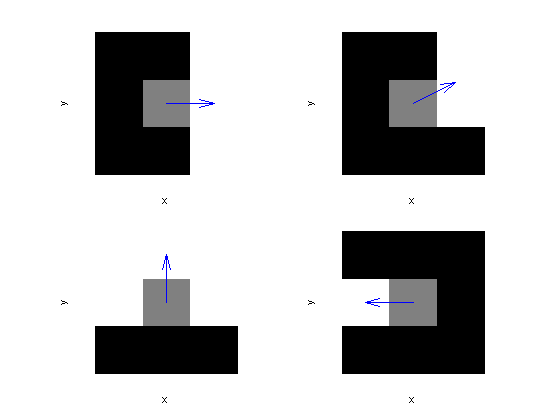
\includegraphics[width=0.9\textwidth, trim=0cm 0cm 0cm 0cm, clip]{DSMC/figures/normal_vectors.png}
\end{center}
\caption{Four different pixels configurations in a $3\times 3$ grid. The filled pixels are marked black whereas the empty pixels are white. We compute the normal vector of the center surface pixels (marked gray) based in its neighbors following equation \eqref{eq:dsmc_normal_vector}. We see that this algorithm generates normal vectors that behave as expected.}
\label{fig:dsmc_normal_vectors}
\end{figure}
In the three dimensional case, we find the normal vectors in exactly the same way, but by using the 26 neighbors. The only thing we need to calculate are the tangent vectors. These can be found by first choosing a random vector $\vec v$ and apply the Gram-Schmidt process making it orthogonal on the normal vector so that
\begin{align}
	\tilde{\vec t}_1 = \vec v - (\vec n\cdot \vec v)\vec n,
\end{align}
which gives the normalized tangent vectors
\begin{align}
	\vec t_1 &= \frac{ \tilde{\vec t}_1}{|\tilde{\vec t}_1|}\\
	\vec t_2 &= \vec n\times \vec t_1.
\end{align}